\documentclass[a4paper]{article}
\usepackage[14pt]{extsizes} 
\usepackage[utf8]{inputenc}
\usepackage[english, russian]{babel}
\usepackage{amsmath}
\usepackage{amsfonts}
\usepackage{amssymb}
\usepackage{graphicx}
\usepackage{indentfirst}
\usepackage{mathtools}
\begin{document}
\begin{center}
\hfill \break
{\large МИНЕСТЕРСТВО НАУКИ ВЫСШЕГО ОБРАЗОВАНИЯ РОССИЙСКОЙ ФЕДЕРАЦИИ}\\
{\large Федеральное государственное бюджетное образовательное учереждение высшего образования}\\
\hfill \break
{\large \textbf{"КУБАНСКИЙ ГОСУДАРСТВЕННЫЙ УНИВЕРСИТЕТ"}} \\
\hfill \break
{\large \underline {Факультет}}\: Математики и Компьютерных Наук\\
{\large \underline {Направление }}\: Математики и Компьютерных Наук\\

\hfill \break
\hfill \break
\hfill \break
{\Large Лабораторная работа №3}\\
{\Large Вариант  №17}\\
\hfill \break \hfill \break
\hfill \break \hfill \break
Работу выполнил \underline{\hspace{7cm}} Батурин Н.Ю.\\
\hfill \break
Специальность \underline{02.03.01 математика и компьютерные науки } курс \underline{ 2}\\
\hfill \break
Специализация \underline{\hspace{11cm}}\\
\hfill \break
Преподаватель \underline{\hspace{6cm}} Виноградова К.Н.\\
\hfill \break
\hfill \break 
\hfill \break \hfill \break
Краснодар\\
2023
\end{center}
\thispagestyle{empty}
\newpage
\begin{center}
\tableofcontents
\end{center}
\newpage
\section{Задание №1} 
\subsection{Условие:}
Определить количество слов в нечётных строках текста.
\subsection{Код:}
\scriptsize
\begin{verbatim}
#include <iostream>
#include <fstream>
#include <string>
using namespace std;
int main() {
    ifstream file("example.txt");
    if (file.is_open()) {
        string word;
        char symbol;
        int kol_str = 1, kol_words = 0;
        while (!file.eof()) {
            file >> word;
            if (kol_str % 2 != 0) kol_words++;
            file.get(symbol);
            if (symbol == '\n') kol_str++;
        }
        cout << "Кол-во слов в нечётных строках:  " << kol_words << endl;
        file.close();
    }
    return 0;
}\end{verbatim}\normalsize
\subsection{Результат:}
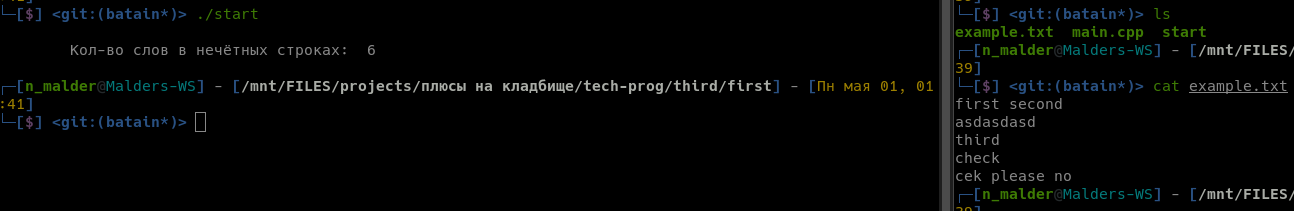
\includegraphics[width=1\textwidth]{1.png}
\newpage
\section{Задание №2} 
\subsection{Условие:}
Даны 3 комплексных числа. Посчитать бех использования библиотеки copmplex x = $\frac{a + b^3 + c}{a - b^2 - c}$
\subsection{Код:}
\scriptsize
\begin{verbatim}
#include <iostream>
using namespace std;
struct Complex { float Im; float Re; };
Complex Plus(Complex first, Complex second) {
    Complex summa;
    summa.Im = first.Im + second.Im;
    summa.Re = first.Re + second.Re;
    return summa;
}
Complex Minus(Complex first, Complex second) {
    Complex difference;
    difference.Im = first.Im - second.Im;
    difference.Re = first.Re - second.Re;
    return difference;
}
Complex Multiply(Complex first, Complex second) {
    Complex piece;
    piece.Re = first.Re * second.Re - first.Im * second.Im;
    piece.Im = first.Re * second.Im + second.Re * first.Im;
    return piece;
}
Complex Share(Complex first, Complex second) {
    Complex division;
    division.Re = (first.Re * second.Re + first.Im * second.Im) / (pow(second.Re, 2) + pow(second.Im, 2));
    division.Im = (second.Re * first.Im - first.Re * second.Im) / (pow(second.Re, 2) + pow(second.Im, 2));
    return division;
}
int main() {
    Complex x, num, den, a, b, c, buffer;
    cout << "Последовательно введите действительную и мнимую часть для\na: ";
    cin >> a.Im >> a.Re;
    cout << "b: "; cin >> b.Im >> b.Re;
    cout << "c: "; cin >> c.Im >> c.Re;
    buffer = Multiply(b, b);
    num = Plus(Plus(a, c), Multiply(buffer, b));
    den = Minus(Minus(a, buffer), c);
    x = Share(num, den);
    cout << "\nX.Re: " << x.Re << "\nX.Im:  " << x.Im << endl;
    return 0;
}\end{verbatim}\normalsize
\subsection{Результат:}
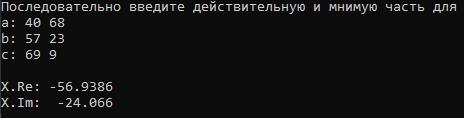
\includegraphics[width=1\textwidth]{2.png}
\newpage
\section{Задание №3} 
\subsection{Условие:}
Для заданных матриц комплексных чисел А(n*n) и B(n*n) найти C = (A^2 + B^2)^T.

Вычислить C^{-1}
\subsection{Код:}
\scriptsize
\begin{verbatim}
#include <iostream>
#include <fstream>
#include <complex>
#include <cmath>
using namespace std;
int SLAU(complex <float>** matrica_a, int n, complex <float>* massiv_b, complex <float>* x){
    int i, j, k, r;
    complex <float> c, M, s;
    float max;
    complex <float>** a, * b;
    a = new complex <float> *[n];
    for (i = 0; i < n; i++)
        a[i] = new complex <float>[n];
    b = new complex <float>[n];
    for (i = 0; i < n; i++)
        for (j = 0; j < n; j++)
            a[i][j] = matrica_a[i][j];
    for (i = 0; i < n; i++)
        b[i] = massiv_b[i];
    for (k = 0; k < n; k++){
        max = abs(a[k][k]);
        r = k;
        for (i = k + 1; i < n; i++)
            if (abs(a[i][k]) > max){
                max = abs(a[i][k]);
                r = i;
            }
        for (j = 0; j < n; j++){
            c = a[k][j];
            a[k][j] = a[r][j];
            a[r][j] = c;
        }
        c = b[k];
        b[k] = b[r];
        b[r] = c;
        for (i = k + 1; i < n; i++){
            for (M = a[i][k] / a[k][k], j = k; j < n; j++)
                a[i][j] -= M * a[k][j];
            b[i] -= M * b[k];
        }
    }
    if (abs(a[n - 1][n - 1]) == 0)
        if (abs(b[n - 1]) == 0)
            return -1;
        else return -2;
    else{
        for (i = n - 1; i >= 0; i--){
            for (s = 0, j = i + 1; j < n; j++)
                s += a[i][j] * x[j];
            x[i] = (b[i] - s) / a[i][i];
        }
        return 0;
    }
    for (i = 0; i < n; i++)
        delete[] a[i];
    delete[] a;
    delete[] b;
}
int INVERSE(complex <float>** a, int n,complex <float>** y){
    int i, j, res;
    complex <float>* b, * x;
    b = new complex <float>[n];
    x = new complex <float>[n];
    for (i = 0; i < n; i++){
        for (j = 0; j < n; j++)
            if (j == i)
                b[j] = 1;
            else b[j] = 0;
        res = SLAU(a, n, b, x);
        if (res != 0)
            break;
        else
            for (j = 0; j < n; j++)
                y[j][i] = x[j];
    }
    delete[] x;
    delete[] b;
    if (res != 0)
        return -1;
    else
        return 0;
}
int main() {
    ifstream size_matrix("matrix_A.txt"), matr_A("matrix_A.txt"), matr_B("matrix_B.txt");
    if (size_matrix.is_open() && matr_A.is_open() && matr_B.is_open()) {
        int size = 0, buf;
        string number;
        char symbol;
        while (symbol != '\n') {
            size_matrix >> number; size++;
            size_matrix.get(symbol);
        }
        size /= 2;
        size_matrix.close();

        complex<float>** A = new complex<float> *[size], ** B = new complex<float> *[size], ** prom_C = new complex<float> *[size], ** C = new complex<float> *[size], ** reverse_C = new complex<float> *[size];
        for (int i = 0; i < size; i++) {
            A[i] = new complex<float>[size];
            B[i] = new complex<float>[size];
            prom_C[i] = new complex<float>[size];
            reverse_C[i] = new complex<float>[size];
            C[i] = new complex<float>[size];
            for (int j = 0; j < n; j++) {
                matr_A >> buf; A[i][j].real(buf);
                matr_A >> buf; A[i][j].imag(buf);
                matr_B >> buf; B[i][j].real(buf);
                matr_B >> buf; B[i][j].imag(buf);
            }
        }
        matr_A.close();
        matr_B.close();
        cout << "A:\n";
        for (int i = 0; i < size; i++) {
            for (int j = 0; j < size; j++) cout << A[i][j] << " ";
            cout << endl;
        }
        cout << "\nB:\n";
        for (int i = 0; i < size; i++) {
            for (int j = 0; j < size; j++) cout << B[i][j] << " ";
            cout << endl;
        }
        cout << "\nC:\n";
        for (int i = 0; i < size; i++)
            for (int j = 0; j < size; j++) {
                A[i][j] *= A[i][j];
                B[i][j] *= B[i][j];
                prom_C[i][j] = A[i][j] + B[i][j];
            }
        for (int i = 0; i < size; i++)
            for (int j = 0; j < size; j++)
                C[j][i] = prom_C[i][j];
        cout << "\nC:\n";
        for (int i = 0; i < size; i++) {
            for (int j = 0; j < size; j++) cout << C[i][j] << " ";
            cout << endl;
        }

        if (!INVERSE(C, size, reverse_C)) {
            cout << endl << "Обратная матрица C:" << endl;
            for (int i = 0; i < size; i++) {
                for (int j = 0; j < size; j++)
                    cout << reverse_C[i][j] << " ";
                cout << endl;
            }
        }

        for (int i = 0; i < size; i++) {
            delete[]A[i];
            delete[]B[i];
            delete[]C[i];
            delete[]prom_C[i];
            delete[]reverse_C[i];
        }
        delete[]A;
        delete[]B;
        delete[]C;
        delete[]reverse_C;
        delete[]prom_C;
    }
    return 0;
}\end{verbatim}\normalsize
\subsection{Результат:}
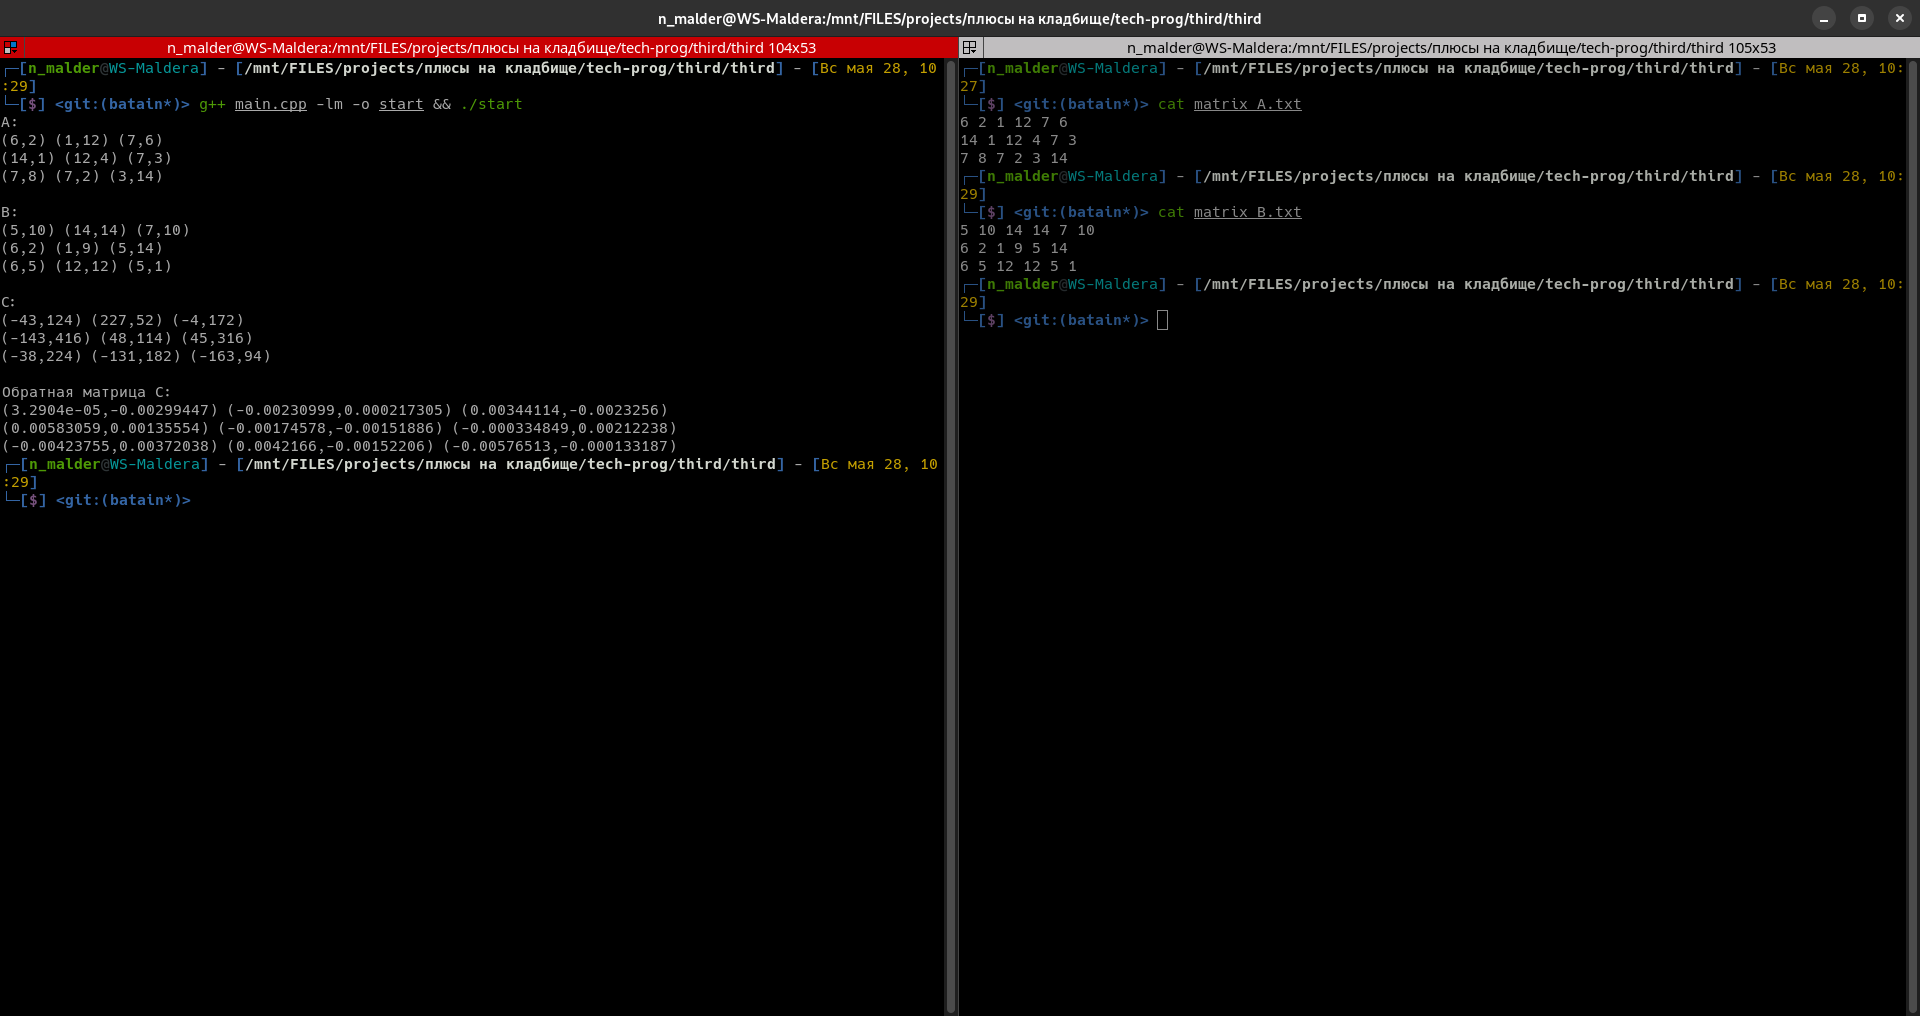
\includegraphics[width=1\textwidth]{3.png}
\subsection{Проверка через мат пакеты:}
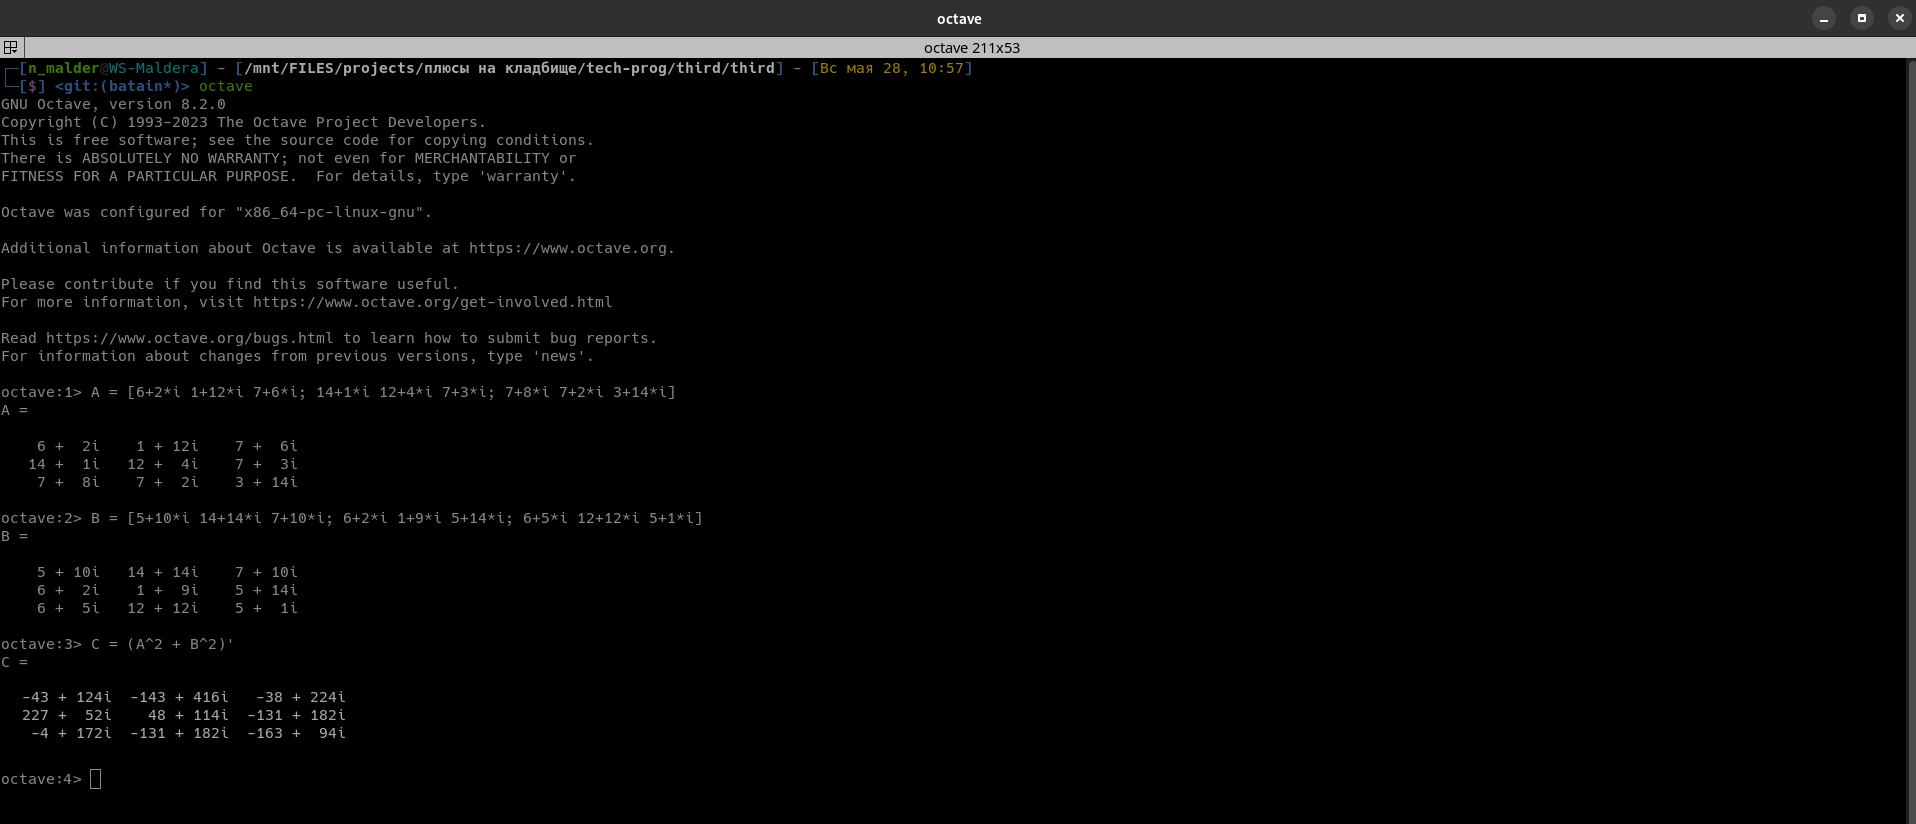
\includegraphics[width=1\textwidth]{check.png}
\end{document}